%-------------------------------------------------------------------------------
%
% TUM Dissertation Template
%
% For usage instructions see README.md
%
% Authors:
%   Andre Richter, andre.richter@tum.de
%   Michael Vonbun, michael.vonbun@tum.de
%   Christian Herber, christian.herber@tum.de
%   Stefan Wallentowitz, stefan.wallentowitz@tum.de
%
%-------------------------------------------------------------------------------
\documentclass[%
  % layouttitlepage,            % layout help rules (to see if you need
  %                             % some extra vspace in your title etc.)
  % headings = standardclasses, % serif fonts for headings
  % headings = big,             % If you use serif fonts for headings (above option
  %                             % uncommmented), uncomment this one to get smaller
  %                             % headings
  % sansseriftitlepage,         % sans serif title page
  % notocintoc,                 % do not add toc to toc itself
]{tumDiss}
\usepackage[utf8]{inputenc}



%-------------------------------------------------------------------------------
% Binding correction for the title page.
% WARNING: ONLY NEEDED FOR THE PRINT VERSION!
%
% After printing and binding, the left part of the titlepage may lose
% significant space, for example due to overlap from glue binding.
% You can increase the left margin of the title page with this option.
% This value of 8mm was measured for glue binding a thesis that was printed by
% the TUM Fachschaft EI and ~140 pages.
%-------------------------------------------------------------------------------
% \titlepagebindingcor{8mm}

%-------------------------------------------------------------------------------
% Binding correction for everything else.
% Does not affect titlePageBindingCor!
%
% WARNING: THIS OPTION CAN SHAKE UP YOUR CURRENT LAYOUT.
% If you want to use it, it is best to work with it from the very start. Adding
% it when finishing your dissertation might get you into trouble.
%
% Search http://texdoc.net/texmf-dist/doc/latex/koma-script/scrguien.pdf for
% "BCOR" for further reading.
%-------------------------------------------------------------------------------
% \KOMAoptions{BCOR=3mm}
% Rename bibliography section


%-------------------------------------------------------------------------------
% Faculty
%-------------------------------------------------------------------------------
%\faculty{Fakultät für Elektrotechnik und Informationstechnik}
\faculty{}

%-------------------------------------------------------------------------------
% Degree
%-------------------------------------------------------------------------------
\degree{Doktors der Naturwissenschaften (Dr. rer. nat.)}

%-------------------------------------------------------------------------------
% Title
%
% IMPORTANT:
%
% You must add manual line breaks here. If you don't, you'll get uneven spacing
% between the lines.
% YOU ALSO NEED THE BREAK AT THE LAST LINE.
%-------------------------------------------------------------------------------
\title{%
  A novel density dependent mechanism of\\
  NPF regulation
}
% \subtitle{That is extended by using an additional subtitle}

%-------------------------------------------------------------------------------
% People
%-------------------------------------------------------------------------------
\author{Ankit Animesh Roy}
% \vorsitz{Prof. Dr.-Ing. Vorname Nachname}
% \erstpruef{Prof. Dr.-Ing. Vorname Nachname}

% Use this one for a TUM professor
% \zweitpruef{Prof. Dr.-Ing. Vorname Nachname}

% Or this one for an external professor
% \zweitpruef[Technische Universität Berlin]{Prof. Dr.-Ing. Vorname Nachname}

% Optionally, add a third examiner
%\drittpruef[RWTH Aachen]{Prof. Dr.-Ing. Max Mustermann}

%-------------------------------------------------------------------------------
% Hand in date
%
% This is the date of your personal hand-in at the TUM doctoral office.
%-------------------------------------------------------------------------------
\date{01.01.2016}

%-------------------------------------------------------------------------------
% Accepted date
%
% You can set this after your thesis was accepted. For handing in,
% it is not needed (at least for the Electrical Engineering faculty).
%-------------------------------------------------------------------------------
\dateaccepted{10.05.2016}



%-------------------------------------------------------------------------------
% Change language, e.g. to german
%-------------------------------------------------------------------------------
% \usepackage[ngerman]{babel}

%-------------------------------------------------------------------------------
% Compatibility issues
%-------------------------------------------------------------------------------
% If you need pstricks, load it here before everything else.
% Otherwise, tikz patterns won't work
%\usepackage{pstricks}

%-------------------------------------------------------------------------------
% Suggested standard packets are included here
%-------------------------------------------------------------------------------
% Loading scrhack fixes:
%   (1) KOMA-Script incompatible macros used in listings package.
%   (2) Inconsistent anchors in hyperref.
\usepackage{scrhack}


% figure inclusion
\usepackage[
  caption = false,
  font    = footnotesize
]{subfig}
\usepackage{graphicx}
\usepackage{pgfplots}
\usepackage{pgfplotstable}
\tikzset{>=stealth}
\usetikzlibrary{patterns}
\usetikzlibrary{pgfplots.statistics}

% code block insertion
\usepackage{moreverb}
\usepackage{listings}

% math and equations
\usepackage{amsmath}
\usepackage{amssymb}
\usepackage{amsfonts}
\usepackage{upgreek}

% enumeration
\usepackage{enumerate}

% Source code with highlighting
\usepackage{listings}
\lstset{
  basicstyle       = \footnotesize,
  captionpos       = b,
  tabsize          = 4,
  commentstyle     = \color{TUMGreen},
  keywordstyle     = \color{TUMBlue},
  stringstyle      = \color{TUMOrange},
  otherkeywords    = {
    uint64_t,
    uint32_t,
    uint16_t,
    uint8_t,
    u64,
    u32,
    u16,
    u8,
    inline
  },
  numbers          = left,
  xleftmargin      = 7ex,
  aboveskip        = 4ex,
  abovecaptionskip = 2ex,
}

% Support for siunitx
\usepackage{siunitx}
\sisetup{
  exponent-product = \cdot,
  output-product   = \cdot,
  per-mode         = symbol-or-fraction,
  quotient-mode    = fraction,
  binary-units     = true
}

% No widows and orphans
\usepackage[all]{nowidow}

% dummy text
\usepackage{lipsum}

% hyperlinks
% according to its documentation, hyperref should be loaded last
% a list of packages that should be loaded after hyperref can be found at
% https://tex.stackexchange.com/questions/1863/which-packages-should-be-loaded-after-hyperref-instead-of-before
\usepackage{url}
\usepackage[
  hidelinks,
  bookmarksnumbered
]{hyperref}

% If hyperref is used, references to tables and figures link to their captions
% and not the actual tables or figures. This is especially unwanted for figures,
% because their captions are below the figure so that clicking on a link just
% shows the captions and the figure is invisible.
%
% Using the caption package fixes this behaviour.
\usepackage{caption}

% glossary functionality
% loading glossaries after hyperref adds hyperlings to acronyms and glossary
% entries
\usepackage[
  toc,
  acronym,
  style = long
]{glossaries}
\makeglossaries

%-------------------------------------------------------------------------------
% Include custom packages here
%-------------------------------------------------------------------------------

\usepackage{setspace}

\setlength{\parskip}{12pt}    % spacing after paragraph
\setlength{\parindent}{0pt}   % paragraph start indentation
\onehalfspacing               % line spacing

%-------------------------------------------------------------------------------
% TUM CI colors for PGF
%-------------------------------------------------------------------------------
\definecolor{grey60} {RGB} {102, 102, 102} % 60% grey

%-------------------------------------------------------------------------------
% Default values for pgfplots
%-------------------------------------------------------------------------------
\newcommand{\figureHeight}{0.5625} %% 16:9
\pgfplotsset{
  compat           = 1.13,
  grid             = major,
  enlarge x limits = 0,
  cycle list name  = tum,
  major grid style = {dotted},
  minor grid style = {dotted},
  legend style     = {
    at     = {(0.98,0.96)},
    anchor = north east,
  },
  width            = \hsize * 0.9,
  height           = \hsize * 0.9 * \figureHeight,
}

%-------------------------------------------------------------------------------
% Rename Bibliography to References
%-------------------------------------------------------------------------------
\renewcommand{\bibname}{References}

%-------------------------------------------------------------------------------
% Correct bad hyphenation here
%-------------------------------------------------------------------------------
\hyphenation{op-tical net-works semi-conduc-tor}

%-------------------------------------------------------------------------------
% Acronyms (will be sorted alphabetically)
%-------------------------------------------------------------------------------
\newacronym{cpu}{CPU}{Central Processing Unit}
\glsadd{cpu}

\newacronym{pci}{PCI}{Peripheral Component Interconnect}
\glsadd{pci}

\newacronym{pcie}{PCIe}{Peripheral Component Interconnect Express}
\glsadd{pcie}

\newacronym{mmu}{MMU}{Memory Management Unit}
\glsadd{mmu}


%-------------------------------------------------------------------------------
% Actual document starts here
%-------------------------------------------------------------------------------
\begin{document}
\frontmatter
\maketitle



%-------------------------------------------------------------------------------
\chapter{Abstract}

\lipsum[1-4]



%-------------------------------------------------------------------------------
\chapter{Zusammenfassung}

\lipsum[1-4]



%-------------------------------------------------------------------------------
\begin{spacing}{0}  % 0 spacing for content and lists
\tableofcontents
\listoffigures
\listoftables
\end{spacing}
\printglossary[type=\acronymtype, nonumberlist]



%-------------------------------------------------------------------------------
\mainmatter
\chapter{Introduction}
\label{chap:introduction}

\lipsum[1-4]



\chapter{State of the Art}
\label{chap:sota}

Example citations~\cite{barham2003xen, LIS}.
Example acronym usage \gls{cpu}.


\chapter{Content}
\label{chap:content}

\lipsum[1]

\section{Example Section}

\lipsum[1-2]
\lipsum[66]



\subsection{Example Table}

\lipsum[1]

\begin{table}[thb]
    \renewcommand{\arraystretch}{1.3}
    \captionabove{Example Table.}
    \label{table:example_table}
    \centering

    \begin{tabular}{|r|l|}
      \hline
      7C0         & hexadecimal \\
      3700        & octal \\
      \cline{2-2}
      11111000000 & binary \\
      \hline
      \hline
      1984        & decimal \\
      \hline
    \end{tabular}
\end{table}


\lipsum[2-4]



\subsection{Example Plot}

\lipsum[1]

\begin{figure}[thb]
    \centering

    \begin{tikzpicture}
        \begin{loglogaxis}[
            xlabel={Degrees of freedom},
            ylabel={$L_2$ Error}
            ]
            \addplot coordinates {
              (5,8.312e-02)    (17,2.547e-02)   (49,7.407e-03)
              (129,2.102e-03)  (321,5.874e-04)  (769,1.623e-04)
              (1793,4.442e-05) (4097,1.207e-05) (9217,3.261e-06)
            };

            \addplot coordinates{
              (7,8.472e-02)    (31,3.044e-02)    (111,1.022e-02)
              (351,3.303e-03)  (1023,1.039e-03)  (2815,3.196e-04)
              (7423,9.658e-05) (18943,2.873e-05) (47103,8.437e-06)
            };

            \addplot coordinates{
              (9,7.881e-02)     (49,3.243e-02)    (209,1.232e-02)
              (769,4.454e-03)   (2561,1.551e-03)  (7937,5.236e-04)
              (23297,1.723e-04) (65537,5.545e-05) (178177,1.751e-05)
            };

            \addplot coordinates{
              (11,6.887e-02)    (71,3.177e-02)     (351,1.341e-02)
              (1471,5.334e-03)  (5503,2.027e-03)   (18943,7.415e-04)
              (61183,2.628e-04) (187903,9.063e-05) (553983,3.053e-05)
            };

            \addplot coordinates{
              (13,5.755e-02)     (97,2.925e-02)     (545,1.351e-02)
              (2561,5.842e-03)   (10625,2.397e-03)  (40193,9.414e-04)
              (141569,3.564e-04) (471041,1.308e-04) (1496065,4.670e-05)
            };

            \addplot coordinates{
              (15,6.75e-02)     (123,3.425e-02)     (745,1.751e-02)
              (5561,5.942e-03)   (30625,2.197e-03)  (90193,9.714e-04)
              (341569,3.564e-04) (871041,1.708e-04) (1896065,8.670e-05)
            };
            \legend{$d=2$,$d=3$,$d=4$,$d=5$,$d=6$,$d=7$}
        \end{loglogaxis}
    \end{tikzpicture}

    \caption{Example Plot.}

    \label{fig:example_plot}
\end{figure}

\lipsum[3]
\lipsum[66]



\subsection{Example Barchart}

\lipsum[1]

\begin{figure}[thb]
    \centering

    \begin{tikzpicture}
        \begin{axis}[
            ybar               = 5pt, % configures `bar shift'
            xmajorgrids        = false,
            x tick label style = {
              /pgf/number format/1000 sep =},
            xtick              = {1930, 1940, 1950},
            ylabel             = y-Axis,
            enlarge x limits   = 0.25,
            ymin               = 2e7,
            ymax               = 8e7,
            bar width          = 9pt,
            point meta         = y *10^-7, % the displayed number
            nodes near coords,
            ]
            \addplot
            coordinates {(1930,70e6) (1940,33e6)
              (1950,40e6)};

            \addplot
            coordinates {(1930,65e6) (1940,42e6)
              (1950,43e6)};

            \addplot
            coordinates {(1930,45e6) (1940,47e6)
              (1950,34e6)};

            \addplot
            coordinates {(1930,34e6) (1940,37e6)
              (1950,38e6)};

            \addplot
            coordinates {(1930,28e6) (1940,27e6)
              (1950,30e6)};

            \addplot
            coordinates {(1930,24e6) (1940,31e6)
              (1950,33e6)};

            \legend{One, Two, Three, Four, Five, Six}
        \end{axis}
    \end{tikzpicture}

    \caption{Example Barchart.}

    \label{fig:example_barchart}
\end{figure}

\lipsum[3]
\lipsum[66]



\subsection{Example SVG Graphics Input}

\lipsum[1]

\begin{figure}[thb]
  \centering
  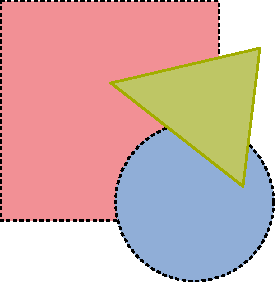
\includegraphics{shapes}

  \caption{Example Shapes from an SVG.}
  \label{fig:example_svg}
\end{figure}

\lipsum[42]



\subsection{Example Source Code}

\lipsum[1]

\begin{lstlisting}[
    language = C,
    caption  = {Example Source Code},
    label    = {list:example_src}
]
#include <stdio.h>

void quick_sort (int *a, int n) {
    int i, j, p, t;
    if (n < 2)
        return;
    p = a[n / 2];
    for (i = 0, j = n - 1;; i++, j--) {
        while (a[i] < p)
            i++;
        while (p < a[j])
            j--;
        if (i >= j)
            break;
        t = a[i];
        a[i] = a[j];
        a[j] = t;
    }
    quick_sort(a, i);
    quick_sort(a + i, n - i);
}

/* main routine */
int main (void) {
    int a[] = {4, 65, 2, -31, 0, 99, 2, 83, 782, 1};
    int n = sizeof a / sizeof a[0];
    int i;
    for (i = 0; i < n; i++)
        printf("%d%s", a[i], i == n - 1 ? "\n" : " ");
    quick_sort(a, n);
    for (i = 0; i < n; i++)
        printf("%d%s", a[i], i == n - 1 ? "\n" : " ");
    return 0;
}
\end{lstlisting}



\subsection{Example Subsection}

\lipsum[1]



\subsubsection{Example SubSubSection}

\lipsum[9]



\subsubsection{Example SubSubSection}

\lipsum[10]



\chapter{Conclusion \& Outlook}
\label{chap:conclusion}

\lipsum[1-4]



%-------------------------------------------------------------------------------
% Bibliography
%-------------------------------------------------------------------------------
%\backmatter
% unsrturl-custom works only with hyperref loaded
% use other styles like unsrt when hyperref is not loaded
\bibliographystyle{unsrturl-custom}
\bibliography{bibliography}



%-------------------------------------------------------------------------------
% Appendix
%-------------------------------------------------------------------------------
\appendix
\chapter{Additional Stuff}

\lipsum[1-4]

\end{document}

%%% Local Variables:
%%% mode: latex
%%% TeX-master: t
%%% End:
